\documentclass[12pt,a4paper,twoside]{report}
\usepackage{cs}
\usepackage{times}
\usepackage{graphicx}
\usepackage{latexsym}
\usepackage{amsmath,amsbsy}
\usepackage{amssymb}
\usepackage[matrix,arrow]{xy}
\usepackage[T1]{fontenc}
\usepackage{ae,aecompl}
\usepackage{amstext}
\usepackage{graphics}
\usepackage[T1]{fontenc}
\usepackage{ae,aecompl}
\usepackage{algorithm}
%\usepackage{algorithmic}
\usepackage{color}
\usepackage{wrapfig}
\usepackage{subcaption}
\usepackage{array}
\usepackage[table]{xcolor}
\usepackage{listings}
\usepackage{xcolor}
\usepackage{float}


\definecolor{codegreen}{rgb}{0,0.6,0}
\definecolor{codegray}{rgb}{0.5,0.5,0.5}
\definecolor{codepurple}{rgb}{0.58,0,0.82}
\definecolor{backcolour}{rgb}{0.95,0.95,0.92}

\lstdefinestyle{codestlye}{
  backgroundcolor=\color{backcolour},
  commentstyle=\color{codegreen},
  keywordstyle=\color{magenta},
  numberstyle=\tiny\color{codegray},
  stringstyle=\color{codepurple},
  basicstyle=\footnotesize,
  breakatwhitespace=false,
  breaklines=true,
  captionpos=b,
  keepspaces=true,
  numbers=left,
  numbersep=5pt,
  showspaces=false,
  showstringspaces=false,
  showtabs=false,
  tabsize=2
}

% \mastersthesis
\diplomathesis
% \leftchapter
\centerchapter
% \rightchapter
\singlespace
% \oneandhalfspace
% \doublespace

\renewcommand{\thesisauthor}{Peter Tibor ZAVACZKI}    %% Your name.
\renewcommand{\thesismonth}{June}     %% Your month of graduation.
\renewcommand{\thesisyear}{2019}      %% Your year of graduation.
\renewcommand{\thesistitle}{FINANCIAL EFFICIENCY BOOSTING SYSTEM FOR CONSUMER-GRADE PRODUCTS}
\renewcommand{\thesissupervisor}{Assoc. Prof. Dr. Eng. Delia Alexandrina MITREA}
\newcommand{\department}{\bf FACULTY OF AUTOMATION AND COMPUTER SCIENCE\\
COMPUTER SCIENCE DEPARTMENT}
\newcommand{\thesis}{LICENSE THESIS}
\newcommand{\utcnlogo}{
\includegraphics[width=15cm]{img/tucn.jpg}}

\newcommand{\uline}[1]{\rule[0pt]{#1}{0.4pt}}
%\renewcommand{\thesisdedication}{P\u{a}rin\c{t}ilor mei}

\begin{document}
%\frontmatter
%\pagestyle{headings}

\newenvironment{definition}[1][Defini\c{t}ie.]{\begin{trivlist}
    \item[\hskip \labelsep {\bfseries #1}]}{\end{trivlist}}



%\thesistitle                    %% Generate the title page.
%\authordeclarationpage                %% Generate the declaration page.

\setcounter{secnumdepth}{3}

\pagenumbering{Roman}
\setcounter{page}{1}

\begin{center}
  \utcnlogo

  \department

  \vspace{4cm}

  {\bf \thesistitle} %LICENSE THESIS TITLE}

  \vspace{1.5cm}

  \thesis

  \vspace{5.75cm}

  Graduate: {\bf \thesisauthor}

  Supervisor: {\bf \thesissupervisor}

  \vspace{3cm}
  {\bf \thesisyear}
\end{center}

\thispagestyle{empty}
\newpage

\begin{center}
  \utcnlogo

  \department

\end{center}
\vspace{0.5cm}

%\begin{small}
\begin{tabular}{p{7cm}p{8cm}}
  %\hspace{-1cm}& APPROVED,\\
  \hspace{-1cm}DEAN,                             & HEAD OF DEPARTMENT,                 \\
  \hspace{-1cm}{\bf Prof. dr. eng. Liviu MICLEA} & {\bf Prof. dr. eng. Rodica POTOLEA} \\
\end{tabular}

% \vspace{2cm}
\vspace{1.6cm}

\begin{center}
  Graduate: {\bf \thesisauthor}

  % \vspace{1cm}
  \vspace{0.6cm}

  {\bf \thesistitle}
\end{center}

\vspace{1cm}

\begin{enumerate}
  \item {\bf Project proposal:} A financial efficiency boosting system for consumer-grade products based on an extension for the Google Chrome browser, webcrawling, a web platform and a RESTful webservice.
  \item {\bf Project contents:} {\it (enumerate the main component parts) Presentation page, advisor's evaluation, title of chapter 1, title of chapter 2, ..., title of chapter n, bibliography, appendices.}
  \item {\bf Place of documentation:} Technical University of Cluj-Napoca, Computer Science Department
  \item {\bf Consultants:} \thesissupervisor
  \item {\bf Date of issue of the proposal:} November 1, 2016
  \item {\bf Date of  delivery:} July 8, 2019
\end{enumerate}

\vspace{1.2cm}
\hspace{6cm} Graduate: \uline{6cm}

\vspace{0.5cm}
\hspace{6cm} Supervisor: \uline{6cm}
%\end{small}

\thispagestyle{empty}


\newpage
$ $
%\begin{center}
%\utcnlogo

%\department
%\end{center}

\thispagestyle{empty}
\newpage

\begin{center}
  \utcnlogo

  \department
\end{center}

\vspace{0.5cm}

\begin{center}
  {\bf
    Declara\c{t}ie pe proprie r\u{a}spundere privind\\
    autenticitatea lucr\u{a}rii de licen\c{t}\u{a}}
\end{center}
\vspace{1cm}



Subsemnatul(a) \textbf{PETER TIBOR ZAVACZKI} legitimat(\u{a}) cu \textbf{C.I.} seria \textbf{MM} nr. \textbf{971552} CNP \textbf{1970131245031}, autorul lucr\u{a}rii \textbf{\thesistitle}
elaborat\u{a} \^{\i}n vederea sus\c{t}inerii examenului de finalizare a studiilor de licen\c{t}\u{a} la Facultatea de Automatic\u{a} \c{s}i Calculatoare, Specializarea \textbf{CALCULATOARE, ENGLEZA} din cadrul Universit\u{a}\c{t}ii Tehnice din Cluj-Napoca, sesiunea \textbf{IULIE} a anului universitar \textbf{2018-2019}, declar pe proprie r\u{a}spundere, c\u{a} aceast\u{a} lucrare este rezultatul propriei activit\u{a}\c{t}i intelectuale, pe baza cercet\u{a}rilor mele \c{s}i pe baza informa\c{t}iilor ob\c{t}inute din surse care au fost citate, \^{\i}n textul lucr\u{a}rii \c{s}i \^{\i}n bibliografie.

Declar, c\u{a} aceast\u{a} lucrare nu con\c{t}ine por\c{t}iuni plagiate, iar sursele bibliografice au fost folosite cu
respectarea legisla\c{t}iei rom\^{a}ne \c{s}i a conven\c{t}iilor interna\c{t}ionale privind drepturile de autor.

Declar, de asemenea, c\u{a} aceast\u{a} lucrare nu a mai fost prezentat\u{a} \^{\i}n fa\c{t}a unei alte comisii de examen de licen\c{t}\u{a}.

\^{I}n cazul constat\u{a}rii ulterioare a unor declara\c{t}ii false, voi suporta sanc\c{t}iunile administrative, respectiv, \emph{anularea examenului de licen\c{t}\u{a}}.

\vspace{1.5cm}

Data \hspace{8cm} Nume, Prenume

\vspace{0.5cm}

\uline{3cm} \hspace{5cm} \textbf{\thesisauthor}

\vspace{0.5cm}
\hspace{9.4cm}Semn\u{a}tura

\thispagestyle{empty}

\newpage

\tableofcontents
\newpage

\pagenumbering{arabic}
\setcounter{page}{1}


\chapter{Introduction - Project Context}
\pagestyle{headings}

The information age has greatly revolutionalized the lives of people all around the globe, bringing along changes that made lives easier, but also more difficult at the same time. The Internet has transformed modern society into homebodies, people who do anything from the comfort of their homes rather than stepping outdoors to complete tasks. People can do it all online : shopping, chatting, paying bills, working, learning, entertaining themselves, even ordering food. Even though life is much simpler than 50 years ago, an average person probably doesn't even know of 50\% of the wonders that the World Wide Web offers them, let alone take advantage of it. That said, an increasing number of individuals use the internet every day to purchase what they need, focusing on the average Joe, who open their browser wishing to buy an item, which, in today's world can be an electronic, articles of clothing, or even groceries. 

According to a statistic published in 2018, there were 1.66 billion individuals engaging in Business-to-Consumer e-commerce, which, considering an approximate 7.55 billion population count of 2017, this would mean that 21.98\% of the global population bought something at least once in 2017 \cite{global_buyers_2017}. According to another statistic, surveying the frequency of purchases made by online shoppers, 20\% of them did online shopping once a week, 25\% once every 2 weeks, 31\% once a month, 15\% 3 to 4 times every 3 months and 10\% once every 3 months \cite{global_frequency_2018}. All these 1.66 billion people, making an average of 2 purchases every month generated 2.3 trillion US dollars of revenue in 2017 and the total revenue generated by e-commerce transactions is predicted to hit 4.9 trillion US dollars by 2021 \cite{global_revenue_2017}.

Humans as consumers, on the other side remained unchanged in two aspects which are relevant to our situation: one being that they will always try to seek the easiest way of doing a task and the other being the nature of constantly trying to spend less on the product they wish to buy. Unfortunately, from these perspectives the modern webshops can be a blessing as much as a burden. They allow you to purchase whatever you need and have it delivered to your doorstep with the minimal amound of physical work necessary. On the other hand they eliminate the option of good old bargaining, but given the vast number of retailers, prices are much more diverse also. And because of the fact that the customer can just as easily click a few times to buy a product from one retailer as from the other, the greatest way for a consumer to save money on their purchase is to find the retailer with the lowest price. As such, people who intend to save some money on their online purchases end up spending valuable amounts of time looking for a product in the webshops they know, which is a very limited number from the ocean of options they would have. These people usually end up just accepting the price they find in the first few webshops to reduce the time they spend shopping. What's more, some actually trustworthy webshops might not even have a very user-friendly interface, often confusing customers when they wish to purchase a product. This means that the probability of finding the lowest price is minimal and the process is extremely time consuming, inefficient and often tiring.

Online retailers, very similarly to their offline counterparts, have a major target in their activities too, that of reaching as many consumers as possible, and creating customers out of them. This, of course can be done via advertisements, but reaching a great amount of people with an advertisement placed on a high traffic website, such as a social network, can be extremely expensive nowadays. Taking into consideration another factor, such as the possible bad reputation the website on which the advertisement appears can also negatively impact the web retailer's or the product's image in the consumer's subconscious. The final, and probably greatest threat to the advertisement based attempts to reach customers is the usage of ad-blocking software, which modify accessed websites' DOM, completely eliminating elements containing advertisements. According to some studies, 236 million desktop users actively used ad-blockig software in December 2016 and 2.3 million mobile users browsing the web from a browser that blocks advertisements by default, majorly due to the fact that 'too many ads are annoying or irrelevant' \cite{adblock_stats}. This means that many users wont even get to see the advertisement the retailer is paying for, and even if they do, it's highly probable that it is of such poor quality or so invasive that the user will just get annoyed by it and he will develop a kind of hate for it.


\chapter{Project Objectives and Specifications}

\section{Introduction}

The purpose of this chapter is to collect, analyze, and define high-level needs and features of this license thesis. It focuses on the capabilities needed by the stakeholders and the target users, and why these needs exist.


\section{Positioning}
\subsection{Problem Statement}

Everyday more and more people are using the internet to buy what they need, from car tires to shoes, from a mobile phone to groceries. Due to the fact that the number of people shopping online increased thus increasing the demand for these opportunities, a naturally companies increased the supply by each creating one or more webshops offering the same product at different prices. This leads to the clients being lost among the options that have, and in a world where you would want to save money at every spending, a tool is necessary for the everyday webshopper to find the best price for their preferred product.

\newcolumntype{g}{>{\columncolor{lightgray}} m{0.45\linewidth}}

\begin{table}[H]
  \centering
  \begin{tabular}{| g | m{0.45\linewidth} |}
    \hline
    \textbf{The problem of}                 & looking for the cheapest offer for a product a client wishes to buy         \\
    \hline
    \textbf{affects}                        & everyday people doing their shopping online                                 \\
    \hline
    \textbf{the impact of which is}         & excessive time spent looking for an offer, ending in unsatisfactory results \\
    \hline
    \textbf{a successful solution would be} &
    easy to use
    easily accessible
    able to track the prices of a set of products across multiple webshops
    easy to extend to cover other webshops
    \\
    \hline
  \end{tabular}
  \label{table:problem_statement}
\end{table}


\subsection{Product Position Statement}

The Financial Efficiency Boosting System (FEBS) comes as a solution to the problem presented in the previous section by the use of webcrawling, a web platform and a Google Chrome extension.

\begin{table}[H]
  \centering
  \begin{tabular}{| g | m{0.45\linewidth} |}
    \hline
    \textbf{For}      & customers of webshops                                                                                           \\
    \hline
    \textbf{who}      & need a tool to simplify their search for a good price                                                           \\
    \hline
    \textbf{The FEBS} & is a system which tracks a set of products on online marketplaces                                               \\
    \hline
    \textbf{that}     & stores current data about products and tells the user about the lowest price of the product they are looking at \\
    \hline
    \textbf{unlike}   & compari.ro                                                                                                      \\
    \hline
    \textbf{The FEBS} &
    will be more accessible                                                                                                             \\
    \hline
  \end{tabular}
  \label{table:product_position_statement}
\end{table}


\section{Stakeholder and User Descriptions}
\subsection{Stakeholder Summary}

\begin{table}[H]
  \centering
  \begin{tabular}{| m{0.3\linewidth} | m{0.3\linewidth} | m{0.3\linewidth} |}
    \hline
    \rowcolor{lightgray} Name & Description                                                       & Responsibilities                                                       \\
    \hline
    \textbf{Webshop customer} & Person who engages in online shopping                             & Find the product they wish to buy and/or track                         \\
    \hline
    \textbf{Online merchant}  & Retailers of products who have their products tracked in the FEBS & Have the data about their products as clear and accessible as possible \\
    \hline
    \textbf{FEBS developer}   & Person who creates and maintains the FEBS                         & Create, improve and offer technical support for the FEBS               \\
    \hline
  \end{tabular}
  \label{table:stakeholder_summary}
\end{table}


\subsection{User Summary}

\begin{table}[H]
  \centering
  \begin{tabular}{| m{0.22\linewidth} | m{0.22\linewidth} | m{0.22\linewidth} | m{0.22\linewidth} |}
    \hline
    \rowcolor{lightgray} Name      & Description                                      & Responsibilities                                                                      & Stakeholder      \\
    \hline
    \textbf{Unregistered customer} & Person who rarely engages in online shopping     & Access the application to find a good offer                                           & Webshop customer \\
    \hline
    \textbf{Registered customer}   & Person who frequently engages in online shopping & Access the application to find a good offer and add products to their favourites list & Webshop customer \\
    \hline
  \end{tabular}
  \label{table:user_summary}
\end{table}


\subsection{User Environment}
\subsubsection{Users}

The application is public and the number of users may fluctuate based on the time of the day/week/month/year. The total number of supported users depends on the server.


\subsubsection{Time limits}

The application should be available all the time, except for maintenance downtimes or unpredictable/uncontrollable downtimes such as power outages. A user can use the application anywhere from a minute if he finds an ideal price to a large time period if they wish to add a product to their favourites list to have it in an easily accessible location.


\subsubsection{Collaboration}

The application is used by a single person, anything a user performs with the system should not influence other users’ experience.


\subsubsection{Infrastructure}

The application will be accessible from web browsers. For full functionality a desktop based Google Chrome will be necessary, as this is the only browser to which an extension will be developed for further ease of use.


\subsection{Summary of Key Stakeholder or User Needs}

\begin{table}[H]
  \centering
  \begin{tabular}{| m{0.18\linewidth} | m{0.08\linewidth} | m{0.18\linewidth} | m{0.26\linewidth} | m{0.21\linewidth} | }
    \hline
    \rowcolor{lightgray} Need                     & Priority & Concerns             & Current solution         & Proposed solution                                        \\
    \hline
    \textbf{Support a multitude of domains}       & 0        & Customers, Merchants & Crawler for each domain  & Analyze and implement a crawler for each new domain      \\
    \hline
    \textbf{Easy to use interface}                & 1        & Customers            & Web platform             & Google Chrome extension which recognizes its environment \\
    \hline
    \textbf{Have an up to date database of items} & 1        & Customers, Merchants & Crawlers for each domain & Run the crawling task at regular intervals               \\
    \hline
  \end{tabular}
  \label{table:summary_of_key_stakeholder_or_user_needs}
\end{table}


\subsection{Alternatives and Competition}

There are similar tools currently available. One of those is compari.ro, which also lists the different webshops and prices for an item, but the fact that a client would have to actually access the website technically makes it harder to use than accessing a Google Chrome extension that is always present and provides data at one click distance.


\section{Product Overview}

The Financial Efficiency Boosting System should provide an easy to use way to users to see the best offer for their desired product. This concept can be seen in figure \ref{fig:system_diagram}.

\begin{figure}[H]
  \centering
  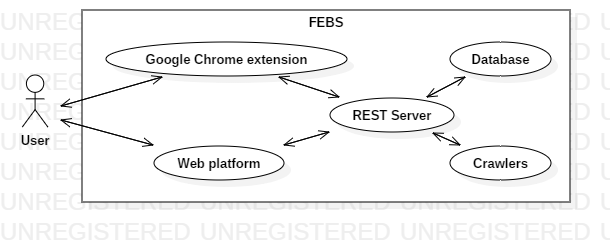
\includegraphics[width=\linewidth]{img/system_diagram.png}
  \caption{The FEBS's system diagram}
  \label{fig:system_diagram}
\end{figure}


\subsection{Product Perspective}

Compared to some competitors, such as compari.ro or PriceMon, FEBS aims to further ease the interaction of the user with the system by offering a font-end through a Google Chrome extension.
FEBS is a standalone application thus it is not part of a larger system.


\subsection{Assumptions and dependencies}

A client is assumed to have a constant internet connection while using the application.

For the server side:

\begin{table}[H]
  \centering
  \begin{tabular}{| m{0.2\linewidth} | m{0.7\linewidth} |}
    \hline
    Database                     & \textbf{MySQL}                                                                                                              \\
    \hline
    Programming language support & \textbf{Java 8}, \textbf{Python 3}, \textbf{Angular 7}                                                                      \\
    \hline
    Frameworks, packages         & for Java: \textbf{Spring framework 2.1.3} or larger, \textbf{MySQL connector 8.0.13}, \textbf{Commons codec 1.12} or larger

    for Python: \textbf{Scrapy 1.6.0} or larger, \textbf{requests 2.22.0} or larger

    for Angular: \textbf{Angular CLI 7.2.4}                                                                                                                    \\
    \hline
    Miscellaneous                & \textbf{Node.js}, \textbf{Node Package Manager (NPM)}                                                                       \\
    \hline
  \end{tabular}
\end{table}

For the client side:

\begin{table}[H]
  \centering
  \begin{tabular}{| m{0.2\linewidth} | m{0.7\linewidth} |}
    \hline
    Web browser & \textbf{Google Chrome 75.0.3770.100} \\
    \hline
  \end{tabular}
\end{table}


\section{Product Features}

\begin{enumerate}
  \item \textbf{Simplistic web platform}

        The web platform should be as simple as possible so that the user can use and navigate it with maximum ease, while still offering the necessary features to accomplish the necessary.

  \item \textbf{Context recognition}

        The Google Chrome extension should automatically check if the user opens a link to a supported domain, in which case it automatically activates in case the user accessed the URL of a supported product it can shows different things if the webshop sells the product at the cheapest price or not: a message stating that the user is looking at the best offer or a link to the product page of the webshop with the cheapest price.

  \item \textbf{Data Monitoring}

        The system tracks changes about the supported products and refreshes the already available information and each distinct running of the respective crawlers.
\end{enumerate}


\section{Other Product Requirements}

\begin{enumerate}
  \item \textbf{Visually minimalist interface}

        The front-end of the application should be as clutter-free as possible, thus improving intuitiveness and ease of use.

  \item \textbf{Usability}

        The application should require close to no input from the user, as it should recognize its working environment to automatically help the user find the cheapest offer. In case user input is necessary, it should be as intuitive as possible to do this, such as interacting with a search bar on the web platform.

  \item \textbf{Performance}

        The system’s performance is measured in the client side response time, which should be at most 5 seconds for most operations.

  \item \textbf{Availability}

        Besides maintenance downtimes, which should take at most 2 hours each week, preferably in a time period when there is as little user activity as possible, there shouldn’t be any availability issue.

  \item \textbf{Scalability}

        The application should be able to serve many concurrent users without introducing too much stress on the system.

  \item \textbf{Maintainability}

        The system should be easily maintained, as most problems could be solved by either rebooting one of the services, or fixing an outdated webcrawler.

  \item \textbf{Extensibility}

        The application should be easily extensible by adding supported products, adding URLs from supported domains to the existing products to gather data about them, or create further crawlers to support more domains.

\end{enumerate}

\chapter{Bibliographic research}
\section{RESTful webservices}
\subsection{The Spring Framework}



\section{Webcrawling}
\subsection{Scrapy}
\subsubsection{Spiders}
\subsubsection{Items and Item Pipelines}


\section{Google Chrome extensions}

\section{Web development}
\subsection{Angular 7}



\chapter{Analysis and Theoretical Foundation}

\section{Conceptual Architecture}


\chapter{Detailed Design and Implementation}



\chapter{Testing and Validation}



\chapter{User's manual}



\chapter{Conclusions}



%\addcontentsline {toc}{chapter}{Bibliography}
\bibliographystyle{IEEEtran}
\bibliography{thesis}%same file name as for .bib

\appendix
\chapter{Relevant code}


\chapter{Other relevant information (demonstrations, etc.)}


\chapter{Published papers}

\end{document}
